\documentclass[french]{book}

\usepackage[top=2cm, bottom=2cm, left=2cm, right=2cm]{geometry}

\usepackage[T1]{fontenc}
\usepackage[utf8]{inputenc}
\usepackage{babel}
\usepackage{pdflscape}
\usepackage{titlesec}
\usepackage{multicol}
\usepackage[inline]{enumitem}
\usepackage{amsmath, amsthm, amssymb}
\usepackage{stackrel}
\usepackage[squaren, Gray]{SIunits}
\usepackage{mathrsfs}
\usepackage{float}
\usepackage{array}
\usepackage{caption}
\usepackage{hyperref} % Liens dans la table des matières


% TikZ

\usepackage{tikz}
\usetikzlibrary{babel}
\usetikzlibrary{calc}
\usetikzlibrary{arrows}
\usetikzlibrary{patterns}
\usetikzlibrary{decorations.pathmorphing, decorations.markings}
\usetikzlibrary{positioning}
\usetikzlibrary{optics}
\usetikzlibrary{shapes.misc}


% "north east hatch" pattern
\makeatletter
\tikzset{% customization of pattern 
        hatch distance/.store in=\hatchdistance,
        hatch distance=5pt,
        hatch thickness/.store in=\hatchthickness,
        hatch thickness=5pt
        }
\pgfdeclarepatternformonly[\hatchdistance,\hatchthickness]{north east hatch}% name
    {\pgfqpoint{-1pt}{-1pt}}% below left
    {\pgfqpoint{\hatchdistance}{\hatchdistance}}% above right
    {\pgfpoint{\hatchdistance-1pt}{\hatchdistance-1pt}}%
    {
        \pgfsetcolor{\tikz@pattern@color}
        \pgfsetlinewidth{\hatchthickness}
        \pgfpathmoveto{\pgfqpoint{0pt}{0pt}}
        \pgfpathlineto{\pgfqpoint{\hatchdistance}{\hatchdistance}}
        \pgfusepath{stroke}
    }
\makeatother

\tikzset{>=stealth}
\tikzset{schema/.style={rounded corners=#1, fill=lightgray, draw, inner sep=0pt},
         schema/.default=4pt}
\tikzset{bati/.style={pattern=north east hatch, hatch distance=7pt, hatch thickness=1.2pt, preaction={fill=lightgray}}}
\tikzset{ressort/.style 2 args={decorate, decoration={coil,aspect=#1,segment length=#2,amplitude=3mm}}}


% Pour les spectres d'émission / d'absorption

\usepackage{pgf-spectra}


% Couverture

\ifpdf
	\usepackage{pdfcolmk}
\fi

\ifxetex
	\usepackage{fontspec}
\fi

\usepackage{url}
\usepackage{graphicx}
\usepackage{pifont}

\newlength{\drop}

\newcommand*{\mytitle}{\begin{titlepage}
\begingroup
\drop = 0.13\textheight
\centering
\vspace*{\drop}
{\Huge Physique (\textsc{mpsi})}\\[\baselineskip]
{\Huge\itshape Année scolaire 2017-2018}\\[3\baselineskip]
{\Large \textit{Cours de} \textsc{N. Tancrez}}\par
\vfill
{\begin{center}\includegraphics[scale=1.5]{SL.png}\end{center}}
\vspace*{1cm}
{\Large Lycée Saint-Louis}\par
\vspace*{\drop}
\endgroup
\end{titlepage}}



% Style des sections

\titleformat{\chapter}
[frame] % format
{\vspace*{5cm}\Huge} % format du texte
{\thechapter} % format du label
{1cm} % séparation
{\centering\sffamily} % avant
[\thispagestyle{empty}] % après


% pour la table des matières
\titleformat{name=\chapter, numberless}
[display] % format
{\Large\bfseries} % format du texte
{\titlerule} % format du label
{-7ex} % séparation
{\centering\MakeUppercase} % avant


\titleformat{\section}
[block] % format
{\LARGE\bfseries} % format du texte
{\thesection} % format du label
{8pt} % séparation
{\centering} % avant

\titleformat*{\subsection}{\Large\bfseries}


\renewcommand{\thechapter}{\Roman{chapter}}
\renewcommand{\thesection}{\arabic{section}.}
\renewcommand{\thesubsection}{\Roman{subsection}}

\pagestyle{plain} % Numéro de page en bas de la page
\setcounter{tocdepth}{1} % On ne veut que les sections

% Math environments

\newtheorem*{lemme}{Lemme}
\newtheorem*{theoreme}{Théorème}
\newtheorem*{propriete}{Propriété}
\newtheorem*{proprietes}{Propriétés}

\theoremstyle{definition}
\newtheorem*{definition}{Définition}
\newtheorem*{definitions}{Définitions}
\newtheorem*{exemple}{Exemple}
\newtheorem*{exemples}{Exemples}
\newtheorem*{experience}{Expérience}
\newtheorem*{vocabulaire}{Vocabulaire}

\theoremstyle{remark}
\newtheorem*{remarque}{Remarque}


% Math macros

\usepackage{mathtools}

\DeclarePairedDelimiter\abs{\lvert}{\rvert}
 
\makeatletter
\let\oldabs\abs
\def\abs{\@ifstar{\oldabs}{\oldabs*}}
\makeatother


\newcommand*\dif{\mathop{}\!\mathrm{d}}


% Conventions du cours

\newcommand*{\point}[1]{\mathrm{#1}}
\newcommand*{\droite}[1]{\mathrm{#1}}
\newcommand*{\systeme}[1]{\mathrm{#1}}
\newcommand*{\vecteur}[1]{\overrightarrow{#1}}
\newcommand*{\algebrique}[1]{\overline{#1}}


\newcommand*{\tdef}[1]{\textbf{#1}}
\newcommand*{\imp}[1]{\emph{#1}}
\newcommand*{\abr}[1]{\textsc{#1}}



% Où chercher les fichiers

\makeatletter
\def\input@path{{01_signaux_harmoniques_propagation/}, {02_optique_geometrique/}}
\makeatother

\newcommand{\cours}[2]
{\begin{landscape}
\begin{multicols*}{2}[\section{#1}]
\input{#2}
\end{multicols*}
\end{landscape}}


%%%%%%% Document %%%%%%%

\begin{document}

% Titre

\mytitle

\tableofcontents

\chapter{\textsc{Signaux harmoniques et propagation}}

\cours{Oscillateur harmonique}{01_oscillateur_harmonique}
\cours{Propagation d'un signal}{02_propagation_signal}
\cours{Ondes progressives sinusoïdales}{03_ondes_progressives_sinusoidales}
\cours{Interférences}{04_interferences}
\cours{Ondes stationnaires}{05_ondes_stationnaires}
\cours{Diffraction}{06_diffraction}

% TODO : ordres de grandeur

\chapter{\textsc{Optique géométrique}}

\cours{Description ondulatoire de la lumière}{01_description_ondulatoire_lumiere}
\cours{Modèle géométrique de la lumière}{02_modele_geometrique_lumiere}
\cours{Systèmes optiques}{03_systemes_optiques}
\cours{Systèmes centrés}{04_systemes_centres}
\cours{Foyers et plans focaux}{05_foyers_plans_focaux}
\cours{Miroir et dioptre plan}{06_miroir_dioptre}
\cours{Lentilles minces sphériques}{07_lentilles_minces_spheriques}
\cours{\abr{lms} dans les conditions de Gauss}{08_lms_conditions_gauss}


\begin{landscape}
\begin{multicols*}{2}[\section{Association de \abr{lms}}]

\subsection{Lentilles de même axe optique}

\begin{propriete}
Si un système optique $\mathscr{S}$ est constitué de $n$ \abr{lms} $\mathscr{L}_1, \ldots, \mathscr{L}_n$ de même axe optique (placés dans cet ordre dans le sens de la lumière incidente), on construit l'image $\point{A'}$ d'un \imp{point objet} $\point{A}$ par $\mathscr{S}$ en construisant les images intermédiaires $\point{A}_1, \ldots, \point{A}_{n-1}$ par les différentes lentilles :
\[\point{A} \stackrel{\mathscr{L}_1}{\longmapsto} \point{A}_1 \stackrel{\mathscr{L}_2}{\longmapsto} \point{A}_2 \stackrel{\mathscr{L}_3}{\longmapsto} \ldots \stackrel{\mathscr{L}_n}{\longmapsto} \point{A'}\]
\end{propriete}

\begin{definition}
Le \tdef{grossissement} optique correspond au rapport entre l’angle $\alpha'$ sous lequel est vue l’image formée par le système optique et l’angle $\alpha$ sous lequel est vu l’objet (par rapport à l'axe optique) :
\[G = \frac{\alpha'}{\alpha}\] 
\end{definition}

\begin{vocabulaire}
On dit que l'image est :
\begin{itemize}
\item \tdef{plus grosse} (resp. \tdef{moins grosse}) que l'objet si $\abs{G} > 1$ (resp. $\abs{G} < 1$);
\item \tdef{droite} (resp. \tdef{renversée}) si $G > 0$ (resp. $G < 0$).
\end{itemize}
\end{vocabulaire}

\begin{exemple}
Une \tdef{lunette de visée à l'infini} sert à observer un objet à l'infini. Pour que l'observation se fasse sans effort (pour un \oe{}il emmétrope), il faut que l'image de cet objet par la lentille soit rejetée à l'infini. C'est donc un système afocal :
\[\point{A}_{\infty} \in \droite{\Delta} \stackrel[\text{objectif}]{\mathscr{L}_1}{\longmapsto} \point{F'}_1 = \point{F}_2 \stackrel[\text{oculaire}]{\mathscr{L}_2}{\longmapsto} \point{A'}_{\infty} \in \droite{\Delta}\]

\begin{figure}[H]
\begin{center}
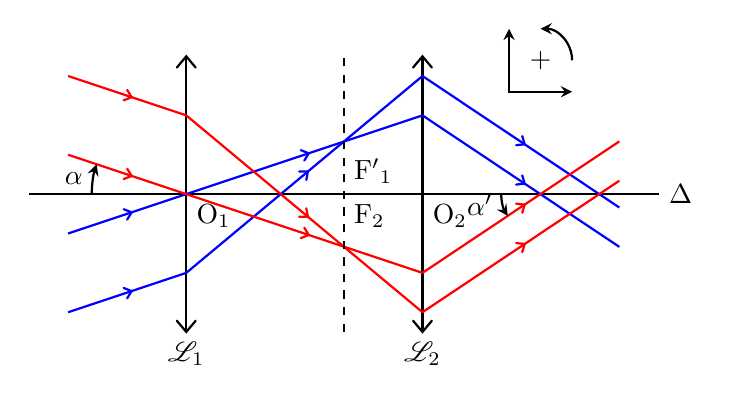
\begin{tikzpicture}[thick, use optics]
\draw (-4,0) -- (4,0) node [right] {$\droite{\Delta}$};

\node[lens, lens type=converging, object height=3.5cm] (L1) at (-2,0) {};
\node [below] at (L1.south) {$\mathscr{L}_1$};
\node [below right] at (L1.center) {$\point{O}_1$};

\node[lens, lens type=converging, object height=3.5cm] (L2) at (1,0) {};
\node [below] at (L2.south) {$\mathscr{L}_2$};
\node [below right] at (L2.center) {$\point{O}_2$};

\draw [blue, ->-] (-3.5,-0.5) -- (-2,0);
\draw [blue, ->-] (-3.5,-1.5) -- (-2,-1);

\draw [blue, ->-] (-2,0)    -- (1,1);
\draw [blue, ->-] (-2,-1)   -- (1,1.5);

\draw [blue, ->-] (1,1) -- (3.5,-0.67);
\draw [blue, ->-] (1,1.5) -- (3.5,-0.17);

\draw [red, ->-] (-3.5,0.5) -- (-2,0);
\draw [red, ->-] (-3.5,1.5) -- (-2,1);

\draw [red, ->-] (-2,0)    -- (1,-1);
\draw [red, ->-] (-2,1)   -- (1,-1.5);

\draw [red, ->-] (1,-1) -- (3.5,0.67);
\draw [red, ->-] (1,-1.5) -- (3.5,0.17);

\draw [->] (-3.2,0) arc (180:161.57:1.2) node [midway, left] {$\alpha$};
\draw [->] (2,0) arc (180:213.69:0.5) node [midway, left] {$\alpha'$};

\draw [dashed] (0,-1.75) -- (0,1.75);
\node [above right] at (0,0) {$\point{F'}_1$};
\node [below right] at (0,0) {$\point{F}_2$};

\node (+) at (2.5,1.7) {$+$};
%\draw [->] (2,1.4) -- node [above] (+) {$+$} +(0.6,0);
\draw [->]  ($ (+) + (0.4,0) $) arc (0:90:0.4);
\draw [<->] ($ (+) + (-0.4,0.4) $) -- ++(0,-0.8) -- +(0.8,0);
\end{tikzpicture}
\end{center}
\end{figure}

\noindent Le grossissement de l'objet observé s'exprime alors :
\[G = -\frac{{f'}_1}{{f'}_2}\]
\end{exemple}



\subsection{Lentilles accolées}

\begin{definition}
Deux \imp{\abr{lms}} sont dites \tdef{accolées} lorsque leurs centres optiques $\point{O}_1$ et $\point{O}_2$ sont confondus :
\[\point{O}_1 = \point{O}_2 = \point{O}\]
\end{definition}

\begin{theoreme}[Lentilles accolées]
Deux \imp{\abr{lms}} $\mathscr{L}_1$ et $\mathscr{L}_2$ \imp{accolées} de vergences $V_1$ et $V_2$ se comportent comme une \abr{lms} $\mathscr{L}$ de vergence $V$ telle que :
\[V = V_1 + V_2\]

\begin{figure}[H]
\begin{center}
\begin{tikzpicture}[thick, use optics]
\coordinate (O1) at (-3.25,0);
\coordinate (O2) at (-2.75,0);
\coordinate (origine) at (-3,0);

\coordinate (O) at (3,0);

\node at (0,0) {$\equiv$};

% Left

\draw (origine) +(-2,0) -- +(2,0) node [right] {$\droite{\Delta}$};

\node[lens, lens type=converging, object height=2.4cm] (L1) at (O1) {};
\node [below left] at (O1) {$\point{O}_1$};

\node[lens, lens type=converging, object height=2.4cm] (L2) at (O2) {};
\node [below right] at (O2) {$\point{O}_2$};

\node [below] at (L1.south) {$\mathscr{L}_1$};
\node [below] at (L2.south) {$\mathscr{L}_2$};

% Right

\draw (O) +(-2,0) -- +(2,0) node [right] {$\droite{\Delta}$};

\node[lens, lens type=converging, object height=2.4cm] (L) at (O) {};

\node [below left] at (O) {$\point{O}$};

\node [below] at (L.south) {$\mathscr{L}$};
\end{tikzpicture}
\end{center}
\end{figure}
\end{theoreme}

\end{multicols*}
\end{landscape}



\chapter{\textsc{Thermodynamique}}

\end{document}
